\section{Architecture}

We describe the architecture of \tl in Figure~\ref{fig:architecture}.
A deep learning developer 
writes a multimedia system using helper functions from \tl.
These functions range from providing and importing layer implementations,
to building neural networks, to managing states involved throughout model life-cycles, 
to creating online or offline datasets, and to writing a parallel training plan.  
These functions are grouped into four modules: layer, network, dataset, and workflow. 
In the following, we describe these modules, respectively.

\begin{figure}
	\centering % trim={<left> <lower> <right> <upper>}
%	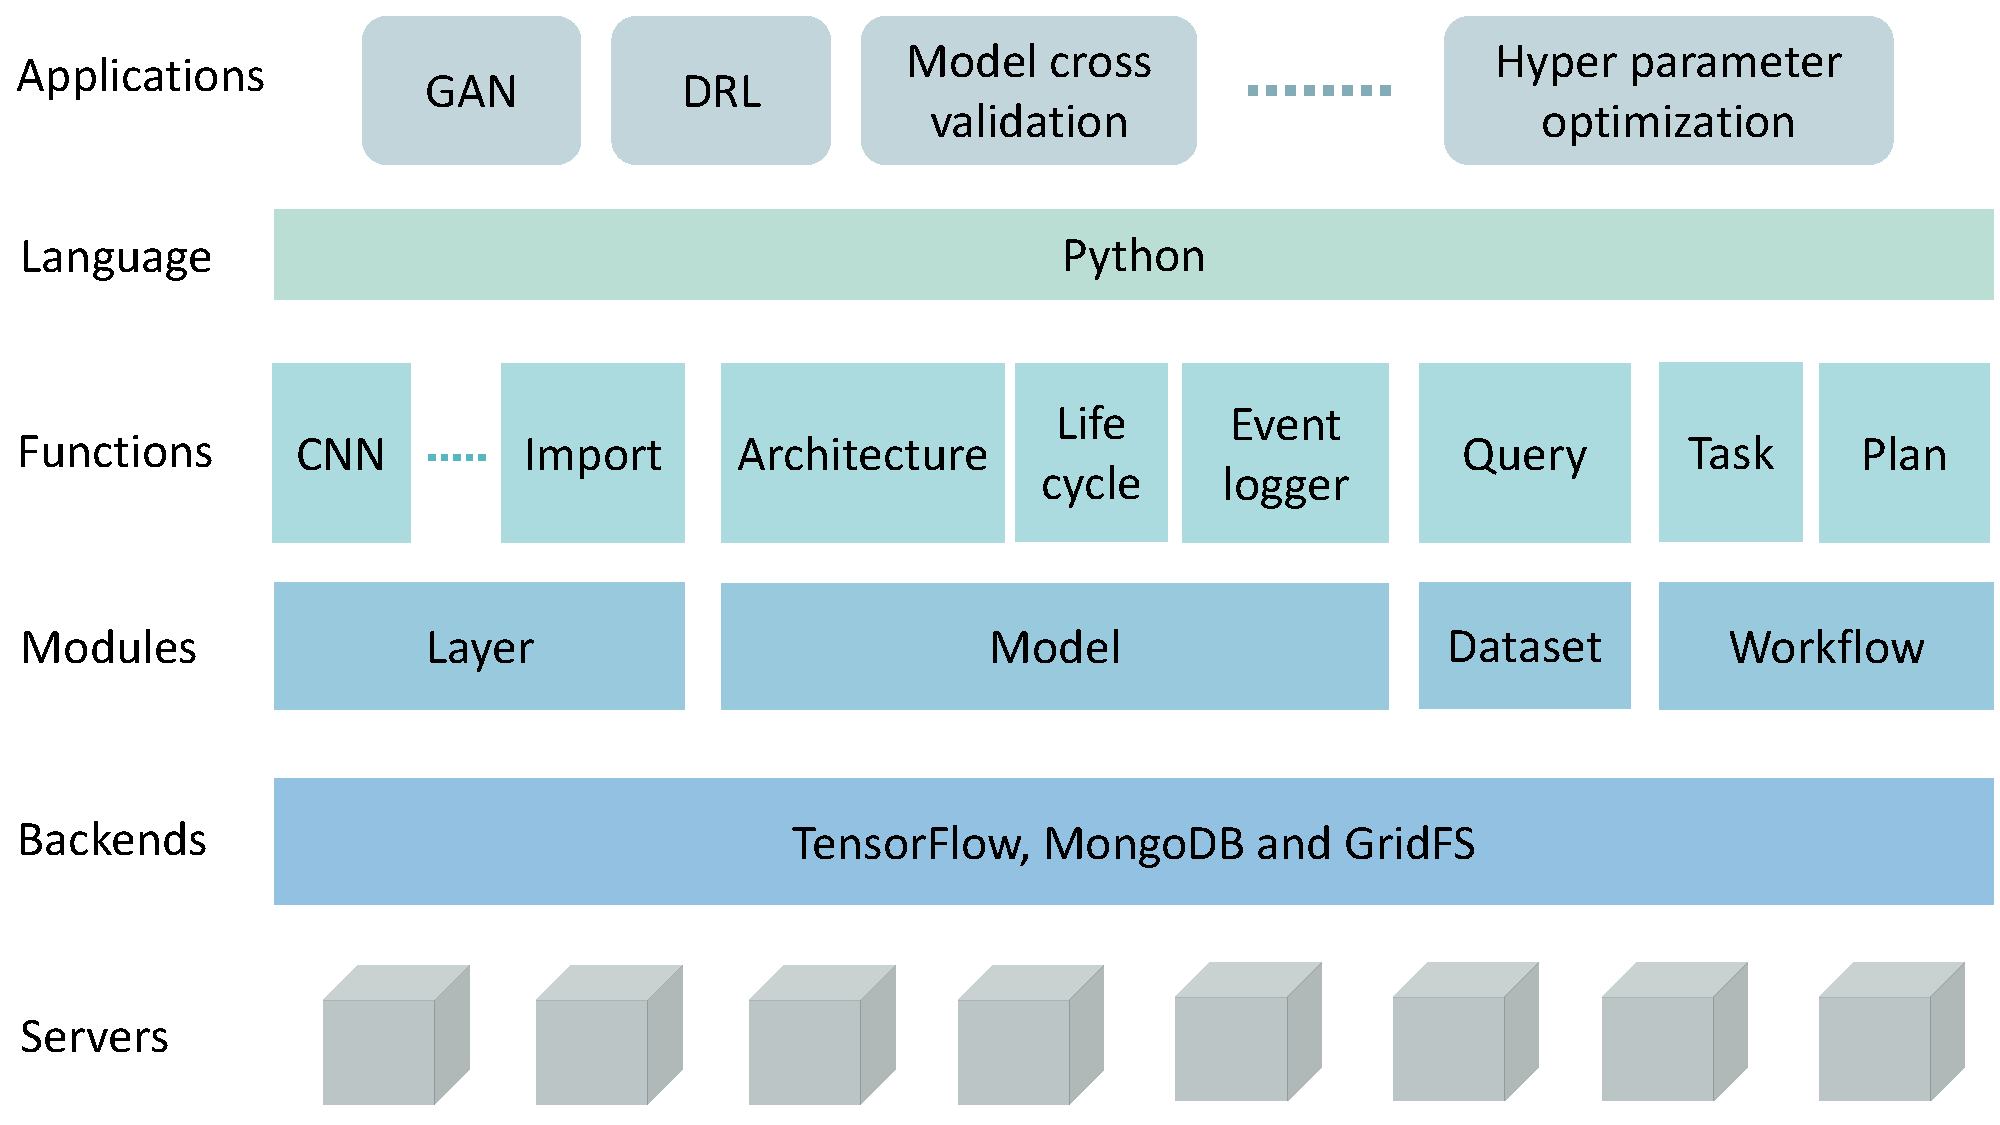
\includegraphics[width=0.46\textwidth]{figures/architecture.pdf}
%	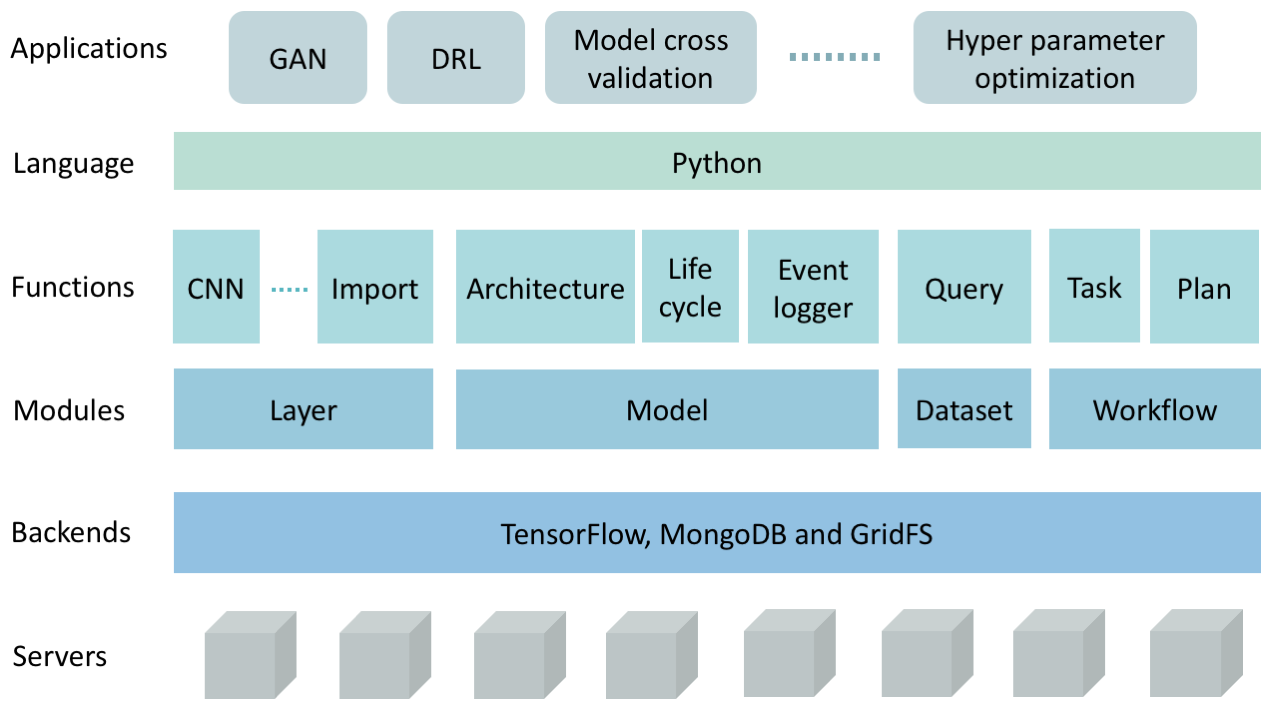
\includegraphics[scale=0.25, trim={0.3cm 0.5cm 0.3cm 0.3cm},clip]{figures/architecture}
	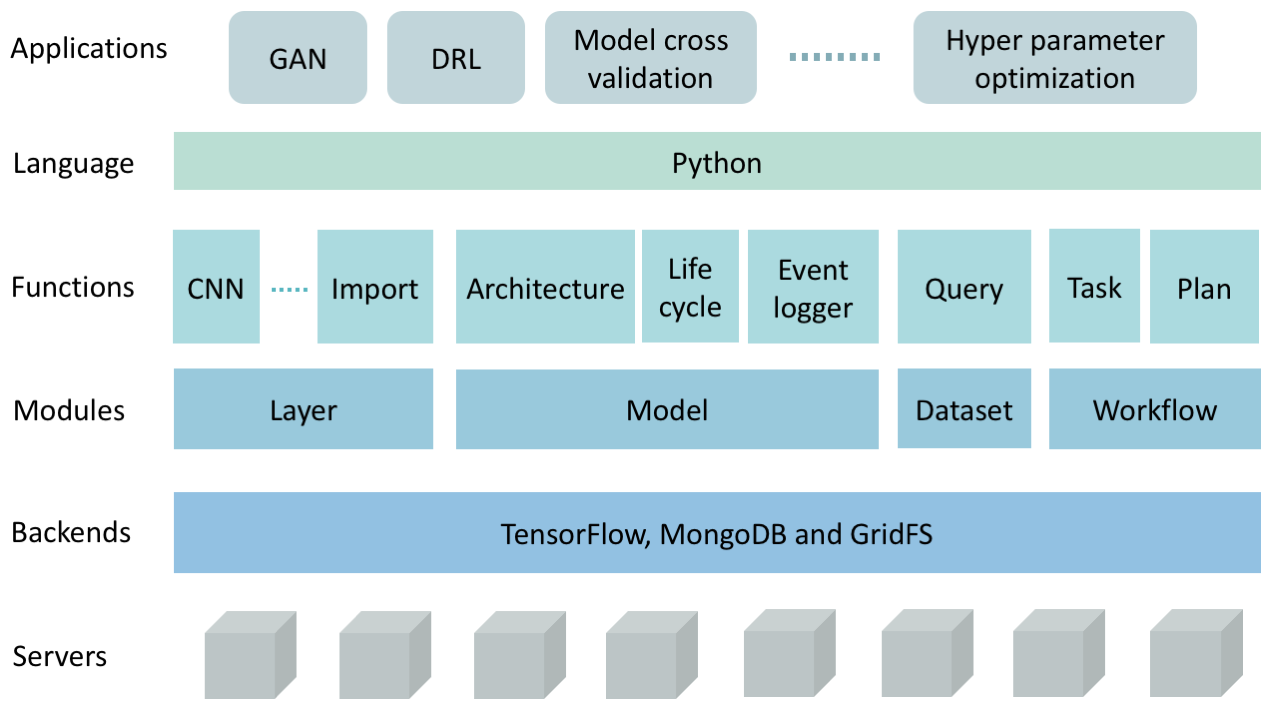
\includegraphics[scale=0.19, trim={0.3cm 0.5cm 0.3cm 0.3cm},clip]{figures/architecture.png}
	\caption{TensorLayer architecture.}
	\label{fig:architecture}
\end{figure} 

\subsection{Layer Module}

Layers are the core bricks of a neural network.
\tl provides a layer module that includes reference implementations of numerous layers, 
such as CNN, RNN, dropout, dropconnect, batch normalization and many others.
Layers are stacked to create a neural network with a declarative fashion, similar to
the extensively used Lasagne~\cite{lasagne}.
Each layer is given an unique key for  
helping developers achieve parameter sharing.
The networks are delegated to TensorFlow.
\tl inherits from TensorFlow to run on hybrid and distributed platforms. 
A concern towards \tl is performance overhead. We investigate this by
running classic models \cite{benchmark} using \tl and native TensorFlow implementations
on a Titan X Pascal GPU. Table~\ref{table:benchmark} shows that \tl exhibits negligible overhead in all models.

\begin{table}[]
	\centering
	\caption{TensorLayer (TL) and TensorFlow (TF) benchmark.}
	\label{table:benchmark}
	\begin{tabular}{|l|l|l|l|}
		\hline
		& CIFAR-10 & PTB LSTM & Word2vec \\ \hline
		TL & 2528 images/s     & 18063 words/s        & 58167 words/s    \\ \hline
		TF  & 2530 images/s    & 18075 words/s      & 58181 words/s   \\ \hline
	\end{tabular}
\end{table}


Layers can be flexibly composed and customized. 
They can be embedded with control functions 
that are lazily evaluated within TensorFlow to adjust training behaviours. This transparency design 
is favoured by \tl users, in particular when they are addressing domain-specific problems that 
require carefully customized models. 
In addition, to ease migration, \tl allows importing external layer and network implementations from other TensorFlow wrappers such as Keras, TFLearn and TFSlim by using the LambdaLayer.

\subsection{Model Module}

Model is the logical representation of a self-contained functional unit, and can be trained, evaluated and deployed in production. Each model has an unique network structure. During training, the model can have different versions or states (i.e., weights).
States can be persisted, cached and reloaded. We use MongoDB as the storage backend. 
Compared to other storage providers such as HBase or MySQL, MongoDB is out-of-box deployable,
simple to use, and rich in third-party management tools. In terms of performance,
it is able to achieve sufficient throughput for processing tensors 
which are the dominant data type in deep learning.

\tl supports recording user-defined model events. Conventional events reflect training steps, learning speed, and accuracy.
They are often used for diagnosing a training process in order to achieve, for example, model versioning~\cite{miao2017modelhub} and interactive learning~\cite{jiang2017interactive}. 

\subsection{Dataset Module}

The dataset module is used for managing training samples and prediction results. 
They are stored as documents in MongoDB. Each document contains a unique key, sample, label and user-defined tags.
Datasets are specified by declarative queries that carry conditions towards tag fields. 
Queries create views of underlying data, and thus do not cost extra storage.

Data are modelled as general streaming datasets. Each dataset is given a \emph{stream}
controller that constantly monitor the availability
of samples and predictions, and then trigger corresponding
training tasks towards this dataset. Intermediate training states are cached in memory
and later reloaded among batches.
The streaming abstraction is able to unify the declaration of offline and online data.
To speed up training efficiency, changes to a dataset is batched until
become significant.

\tl optimizes dataset performance thoroughly. Firstly, 
\tl creates indexes for frequently visited tags to accelerate
row selection. Secondly, datasets can be cached locally and partitioned to distribute workloads.
Thirdly, chunky data are compressed and sent in 
batches to improve I/O efficiency. Thirdly, in addressing
big blobs such as videos, \tl
adopts GridFS as the blob store.
In such a case, the rows in MongoDB carry pointers to the locations of sample blobs in GridFS. 
This two-layer storage architecture is transparent to developers. 

\subsection{Workflow Module}

The workflow module provides task abstraction to enable fault-tolerant asynchronous training. 
A training task is uniquely identified by 3-tuple: an input dataset key, a model key, and an output dataset key.
It is inserted into a task queue subscribed by an agent. An agent can
perform CPU / GPU training task or any user-defined function written in Python. Task completion messages are published onto a notification
queue subscribed by an agent master. 
This pub-sub system is naturally asynchronous. Multiple tasks can form a training plan to be scheduled by the master. Queues are persisted in the storage backend to ensure that failed tasks are replayed.

The workflow module simplifies the implementation of model group operations and learning systems that involves asynchronous feedback loops in operation. It is also 
useful for complex cognitive systems
that have training dependency among components. 
For example, the developer of an image captioning system \cite{showandtell2015} first trained
a CNN to understand the context of images, and then trained a
RNN decoder to generate description based on recognized context. This example
thus forms a two-stage asynchronous training plan that can be supported by \tl.



















